\chapter{Results}
Here the results of the implemented control strategies developed in \textit{Part 1} are presented. Firstly, the swing-up controller is approaching a heteroclinic orbit after seven swings, see \autoref{fig:theta_swing_p00} and \ref{fig:x_swing_p00}, same as achieved in simulation when accounting for actuation limitations.
%ADDITIONAL PLOTS AVAILABLE
%
%thetaDot_swing_p00
%xDot_swing_p00
%thetaDotBiasZoom_swing_p00
%
\begin{figure}[H]
  \hspace{1cm}
  \captionbox
  {
    The swing-up controller approaches the equilibrium and eventually reaches the heteroclinic orbit.
    \label{fig:theta_swing_p00}
  }
  {
    \hspace{-1cm}
    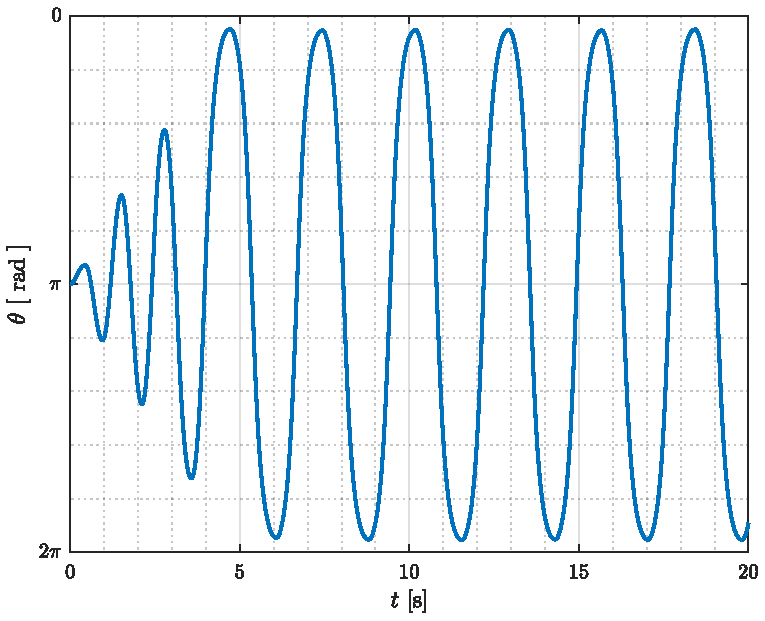
\includegraphics[width=.39\textwidth]{figures/theta_swing_p00}
  }
  \hspace{20pt}
  \captionbox 
  {
    Once the energy reference is tracked, the cart maintains a closer proximity to zero on the rail.
    \label{fig:x_swing_p00}
  }
  {
    \hspace{-1cm}
    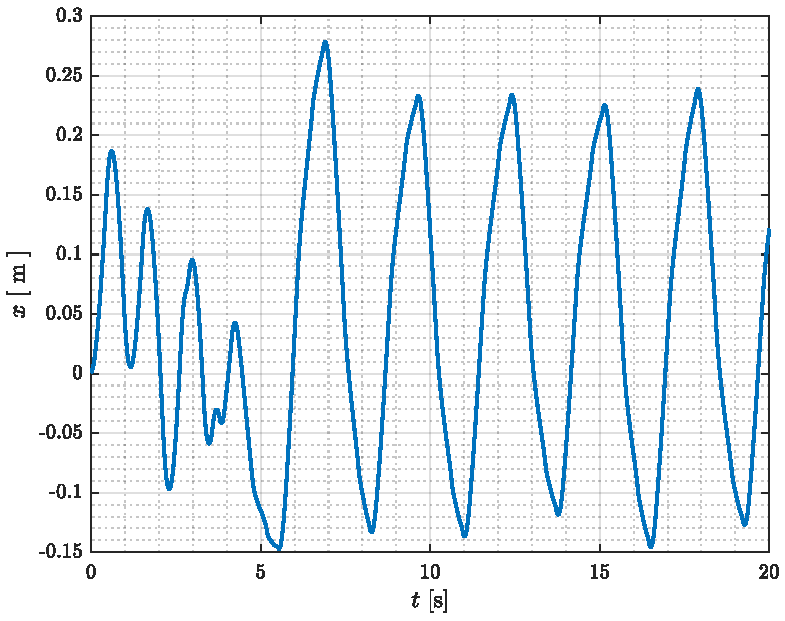
\includegraphics[width=.4\textwidth]{figures/x_swing_p00}
  }  
\end{figure}
%
The controller does fall slightly short of reaching the heteroclinic orbit which is also seen in \autoref{fig:phase_swing_p00}. The energy reference in \autoref{fig:Edelta_swing_p00} reaches zero near the equilibrium points, but must be very slightly below zero when the angular velocity is zero, as otherwise the pendulum would reach equilibrium exactly.
\begin{figure}[H]
  \hspace{1cm}
  \captionbox
  {
    From the test in \autoref{fig:theta_swing_p00} and \ref{fig:x_swing_p00} energy reference is reached.
    \label{fig:Edelta_swing_p00}
  }
  {
    \hspace{-1cm}
    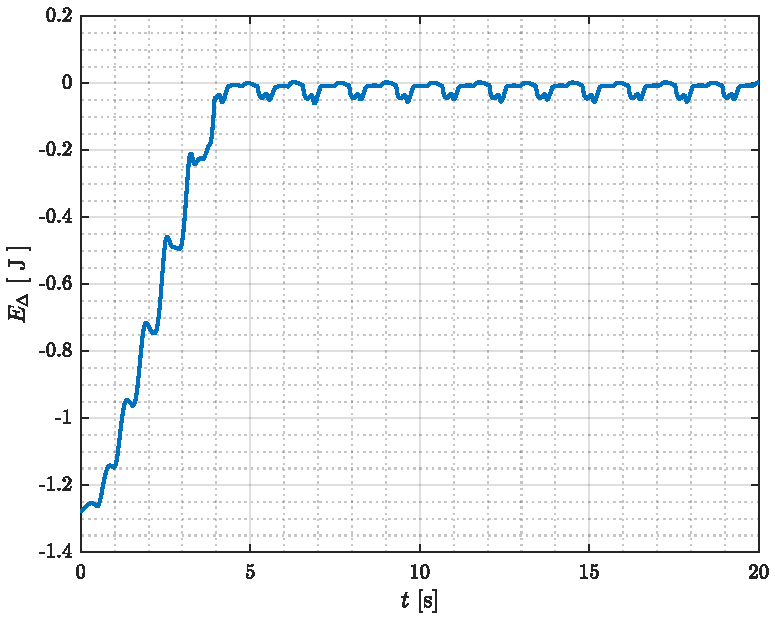
\includegraphics[width=.4\textwidth]{figures/Edelta_swing_p00}
  }
  \hspace{20pt}
  \captionbox 
  {
    The pendulum almost reaches a heteroclinic orbit.
    \label{fig:phase_swing_p00}
  }
  {
    \hspace{-1cm}
    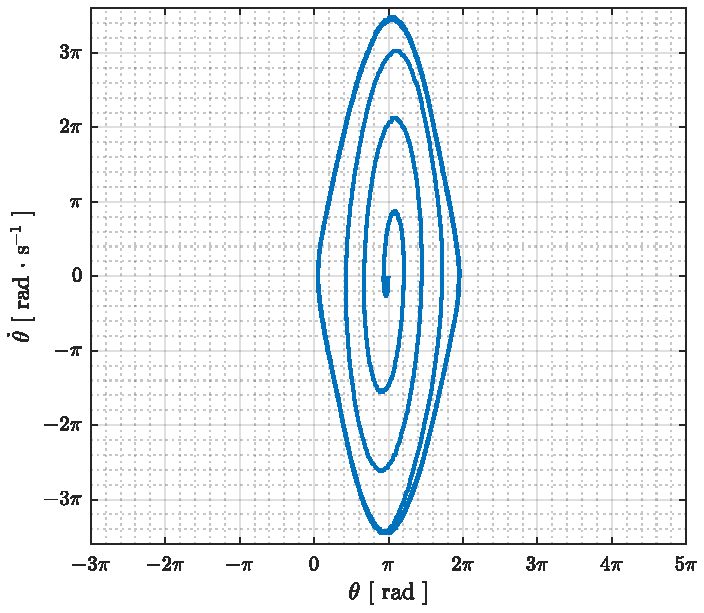
\includegraphics[width=.364\textwidth]{figures/phase_swing_p00}
  }  
\end{figure}
%
%\begin{figure}[H]
%  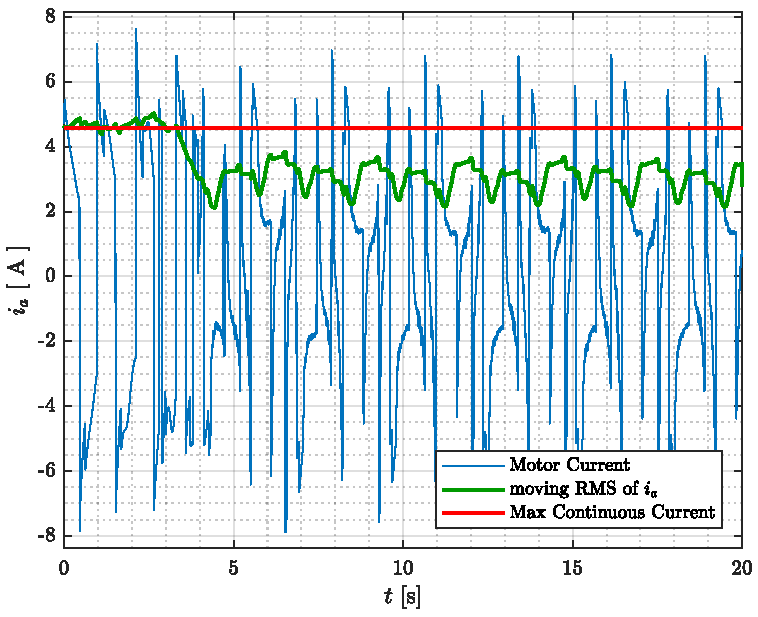
\includegraphics[width=.42\textwidth]{figures/ia_swing_p00}
%  \caption{ ia swing p00 }
%  \label{fig:ia_swing_p00}
%\end{figure}
%
It is possible to gain closer proximity to the equilibrium point by increasing the energy reference. In \autoref{fig:theta_swing_p08} and \ref{fig:x_swing_p08} the energy reference is increased by \SI{0.08}{J} to reach heteroclinic orbit.
%
%ADDITIONAL PLOTS AVAILABLE
%
%thetaDot_swing_p08
%xDot_swing_p08
%thetaDotBiasZoom_swing_p08
%
\begin{figure}[H]
  \hspace{1cm}
  \captionbox
  {
    The swing-up controller approaches the equilibrium and eventually reaches the heteroclinic orbit.
    \label{fig:theta_swing_p08}
  }
  {
    \hspace{-1cm}
    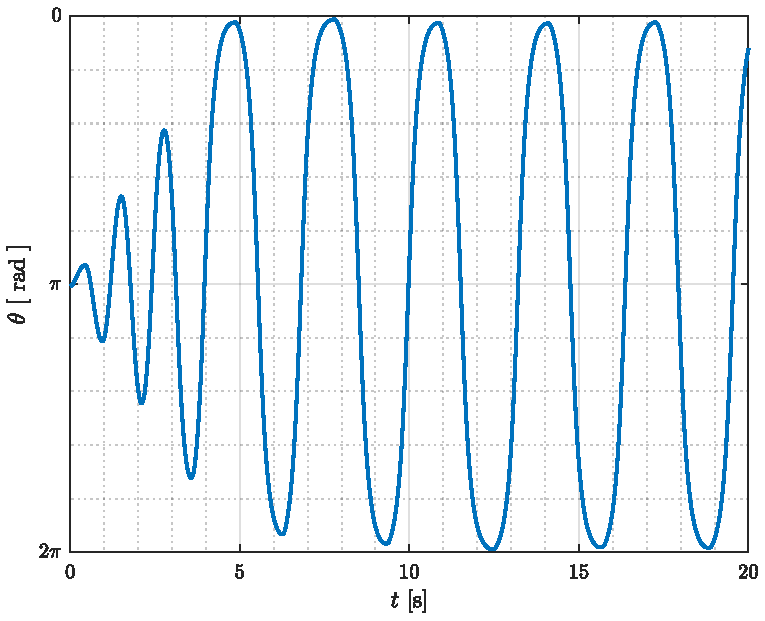
\includegraphics[width=.395\textwidth]{figures/theta_swing_p08}
  }
  \hspace{20pt}
  \captionbox 
  {
    The cart does not approach zero position as much as it did in simulation. It does however stay within the constraints of the physical system, which is the main objective of the added position control for the swing-up sequence.
    \label{fig:x_swing_p08}
  }
  {
    \hspace{-1cm}
    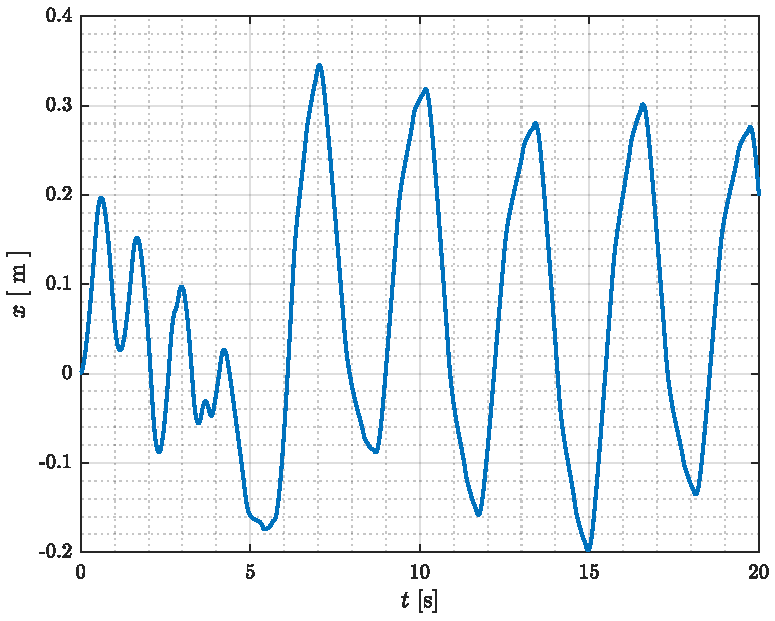
\includegraphics[width=.4\textwidth]{figures/x_swing_p08}
  }  
\end{figure}
In \autoref{fig:Edelta_swing_p08} the energy reference is slightly lifted causing a near perfect heteroclinic orbit in \autoref{fig:phase_swing_p08}.
\begin{figure}[H]
  \hspace{1cm}
  \captionbox
  {
    From the test in \autoref{fig:theta_swing_p08} and \ref{fig:x_swing_p08} where the energy reference is raised by \SI{0.08}{J} to get closer to the equilibrium point.
    \label{fig:Edelta_swing_p08}
  }
  {
    \hspace{-1cm}
    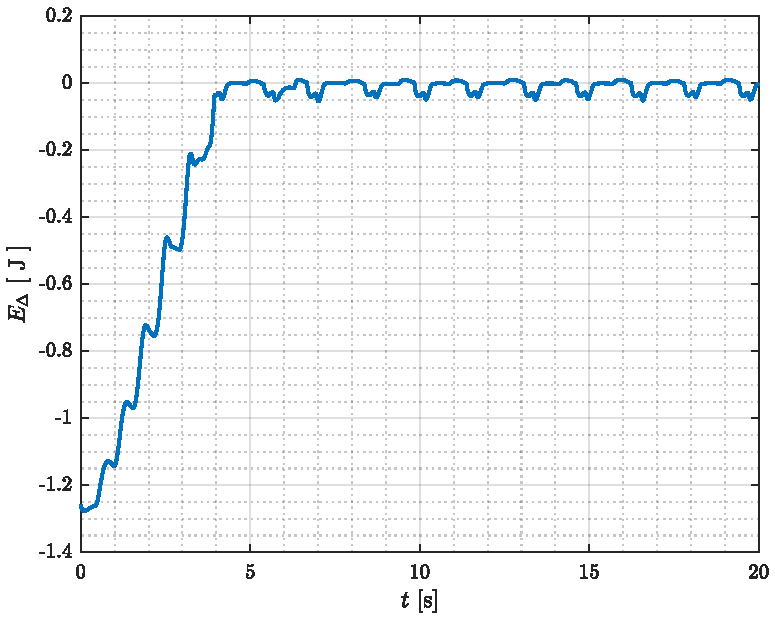
\includegraphics[width=.4\textwidth]{figures/Edelta_swing_p08}
  }
  \hspace{20pt}
  \captionbox 
  {
    Near perfect heteroclinic orbit is reached due to the slight increase of the energy reference.
    \label{fig:phase_swing_p08}
  }
  {
    \hspace{-1cm}
    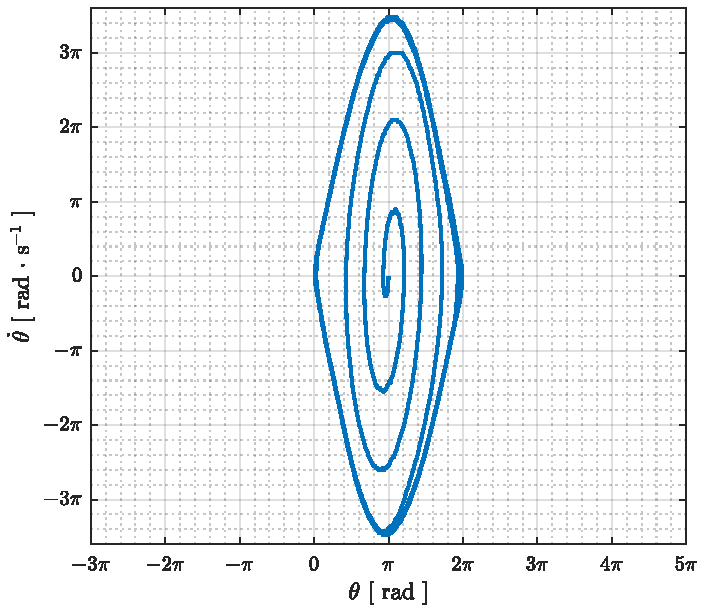
\includegraphics[width=.364\textwidth]{figures/phase_swing_p08}
  }  
\end{figure}
If the model and friction compensation was ideal, no energy offset would be needed, so if a high value were needed to approach equilibrium it might be worth to revisit this part of the design process.
%
\autoref{fig:ia_swing_p08} shows the armature current of the motor used to achieve the swing-up behavior with the added energy reference. Though some peaks are present in the current signal, the moving RMS value does not exceed the continuous current specification of the motor for extended periods of time.
\begin{figure}[H]
  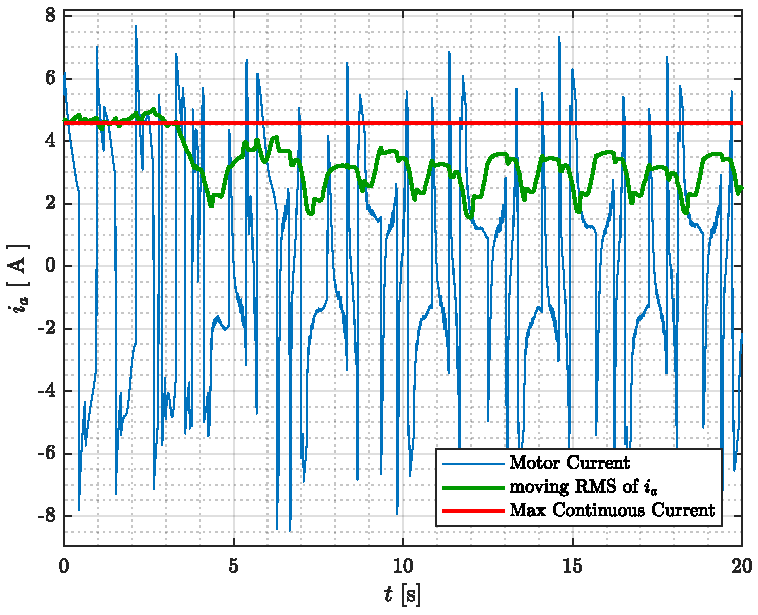
\includegraphics[width=.42\textwidth]{figures/ia_swing_p08}
  \caption{The moving RMS of the armature current is withing respectable levels of the specified contentious current limit of the motor.}
  \label{fig:ia_swing_p08}
\end{figure}
%
A test of the implemented sliding mode controller is seen in \autoref{fig:theta_slide} and \ref{fig:x_slide} where the angle reaches zero.
%ADDITIONAL PLOTS AVAILABLE
%
%thetaDot_slide
%xDot_slide
%thetaDotBiasZoom_slide
\begin{figure}[H]
  \hspace{1cm}
  \captionbox
  {
    Test of sliding mode controller starting at zero. The controller is subjected to a disturbance after which it rebalances successfully bringing the angle back to zero.
    \label{fig:theta_slide}
  }
  {
    \hspace{-1cm}
    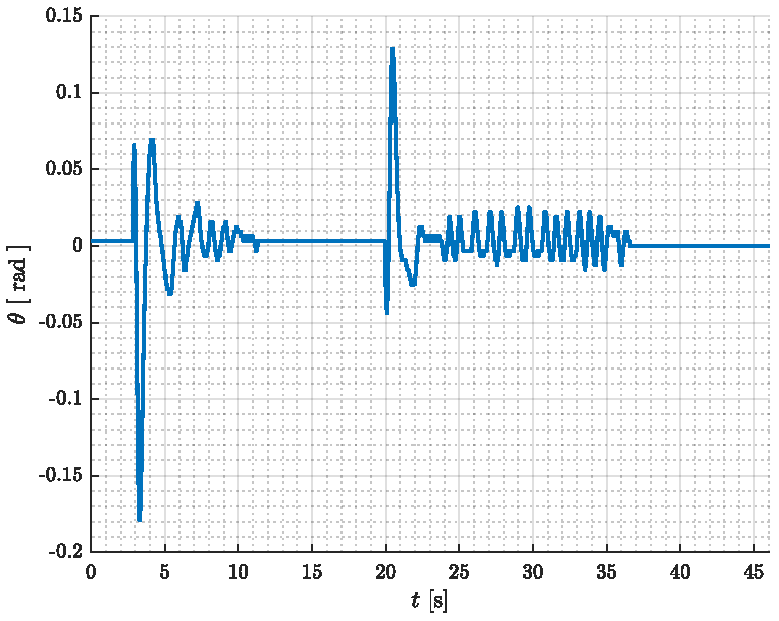
\includegraphics[width=.4\textwidth]{figures/theta_slide}
  }
  \hspace{20pt}
  \captionbox 
  {
    The cart returns to zero once the pendulum is rebalanced.
    \label{fig:x_slide}
  }
  {
    \hspace{-1cm}
    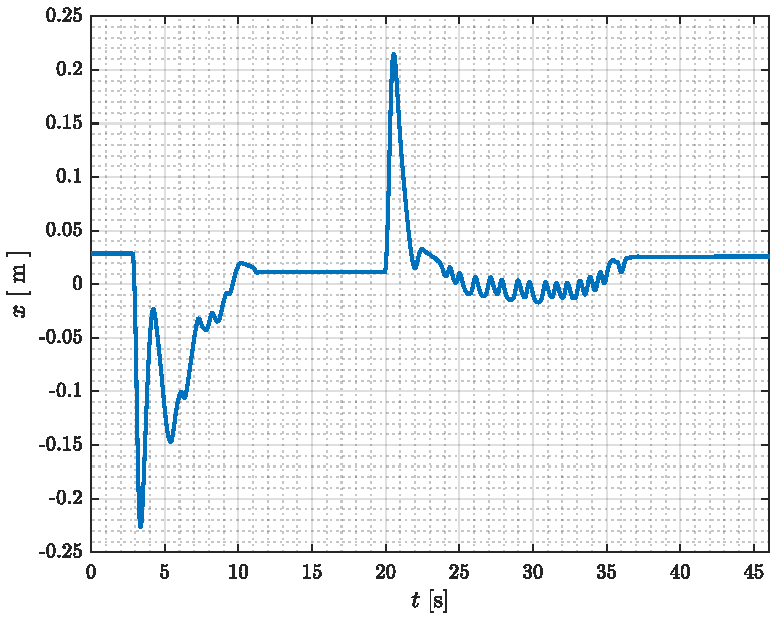
\includegraphics[width=.4\textwidth]{figures/x_slide}
  }  
\end{figure}
In the last part after the \SI{35}{s} mark a rather large offset in $x$ is observed, this could be contributed to unmodeled friction keeping the control from exceeding the force of friction. The control signal is shown in \autoref{fig:ia_slide} where it does have a constant offset after the \SI{35}{s} mark, supporting the hypothesis. However, some offset is also seen in the other stabilized regions of the test, where the control signal goes to zero. So while the first hypothesis might in part be true, something else is at least contributing to the problem, otherwise the control would still show an offset where the cart position does.
%
\begin{figure}[H]
  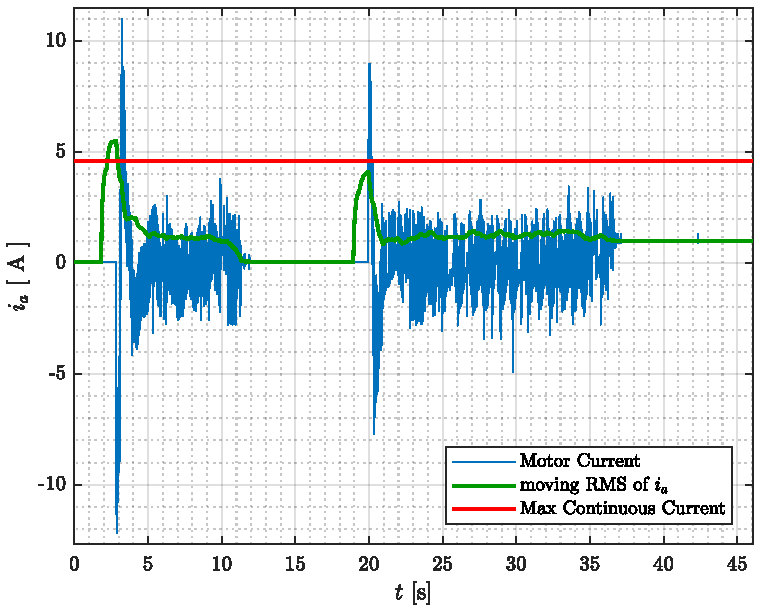
\includegraphics[width=.42\textwidth]{figures/ia_slide}
  \caption{ ia slide  }
  \label{fig:ia_slide}
\end{figure}
%
When testing an other problem relating to the position of the cart was observed. In \autoref{fig:states_slideEKFproblem} the pendulum is only pushed once in the start of the test. The cart spontaneously diverges from zero position before correcting and re-stabilizing. When this happens, the angular velocity should not increase much, as seen by the FIR filter, which by nature does not introduce bias, however, the EKF shows an increase in angular velocity.
%
\begin{figure}[H]
  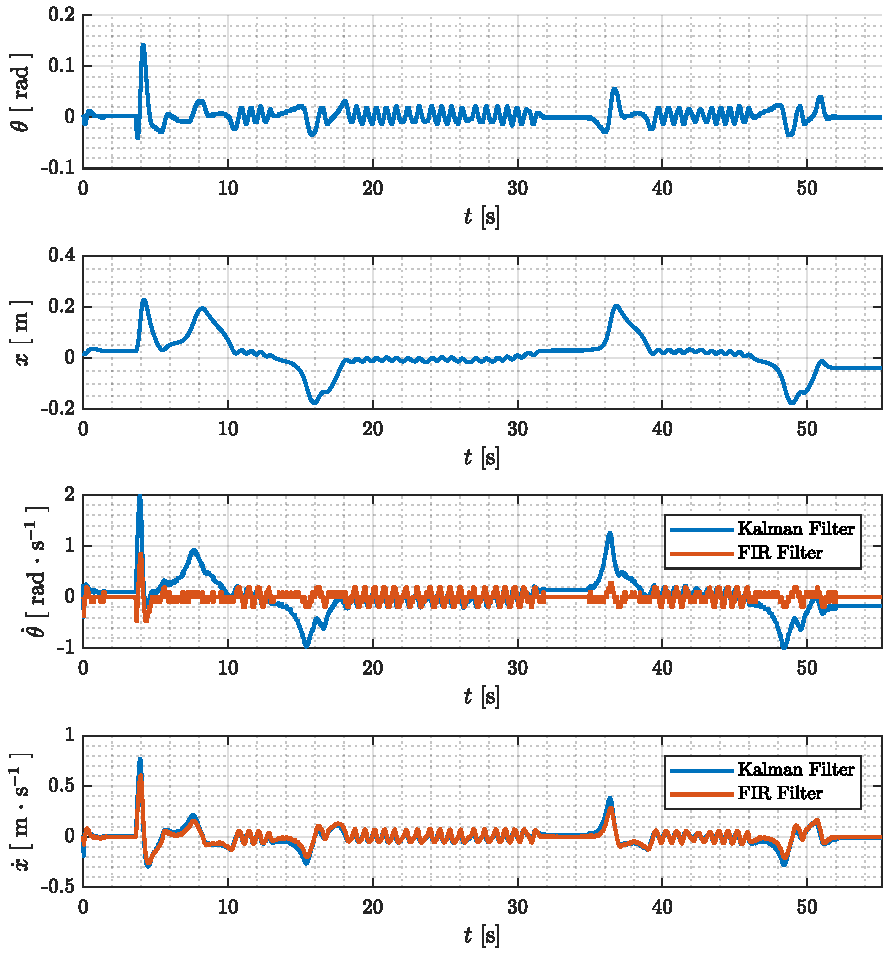
\includegraphics[width=.7\textwidth]{figures/states_slideEKFproblem}
  \caption{The system is perturbed about \SI{35}{s} into the test, remaining disturbances are caused by a problem presumed to arise between friction compensation and the EKF.}
  \label{fig:states_slideEKFproblem}
\end{figure}
If the friction compensation is too large, this could cause the cart to move away from equilibrium, and in that event, the EKF which is based on a system model, would get data which does not confine to the model, which might lead to a wrong estimation of the angular velocity, which would then amplify the problem.
%

When finally combining the two control strategies it is advantageous for the catch controller if the swing-up controller is designed to provide a bit of entry velocity at equilibrium. This makes for a more robust swing-up controller, in that, it always reaches the equilibrium in the same number of swings for every test. This means that the swing-up controller would overshoot without a catch controller. However, as the catch controller is enabled close to equilibrium, this helps the sliding mode controller by providing entry velocity at the maximum catch angle.\\
It is further noted that smaller catch angles causes less aggressive actuation of the sliding mode controller. After entering sliding mode the catch angle is increased, such that it stays in sliding mode unless the pendulum exceeds the maximum angle at which sliding mode can successfully re-stabilize the system. When this angle is exceeded, the swing-up controller is enabled and the catch angle is reduced. As in simulation, a wrapped version of the angle is created such that the pendulum is always at zero when in upright position, this representation is only used by sliding mode.\\
Results of a test of the full implementation of the two controllers is shown in \autoref{fig:theta_swingNslide} and \ref{fig:x_swingNslide}.
%
%ADDITIONAL PLOTS AVAILABLE
%
%thetaDot_swingNslide
%xDot_swingNslide
%phase_swingNslide
%Edelta_swingNslide
\begin{figure}[H]
  \hspace{1cm}
  \captionbox
  {
    Test of the final design of swing-up with the higher energy reference and sliding mode controller successfully catching the pendulum after seven swings.
    \label{fig:theta_swingNslide}
  }
  {
    \hspace{-1cm}
    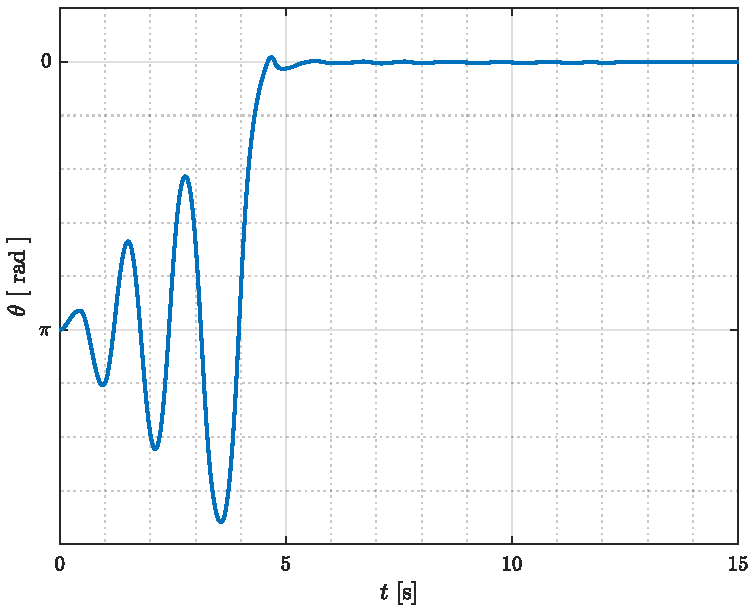
\includegraphics[width=.384\textwidth]{figures/theta_swingNslide}
  }
  \hspace{20pt}
  \captionbox 
  {
    The cart keeps around zero on the rail, especially after the pendulum angle is controlled to zero.
    \label{fig:x_swingNslide}
  }
  {
    \hspace{-1cm}
    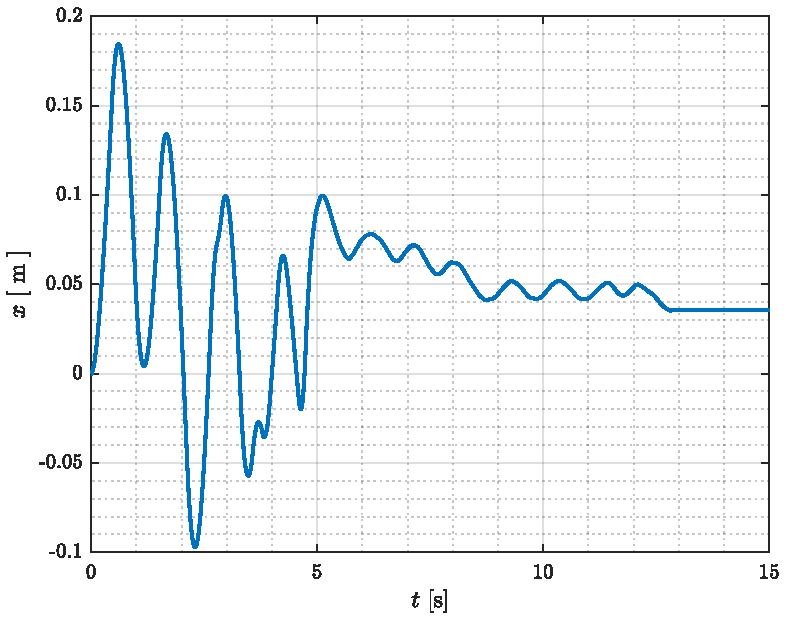
\includegraphics[width=.4\textwidth]{figures/x_swingNslide}
  }  
\end{figure}
The swing-up controller successfully hands over to sliding mode after seven swings and the sliding mode controller stabilizes the system in zero with some offset in the cart position.
The moving RMS of the actuation current briefly exceeds the continuous current rating of the motor when sliding mode catches the pendulum. As this is not happening over a prolonged period, it is not thought to be a problem,
\begin{figure}[H]
  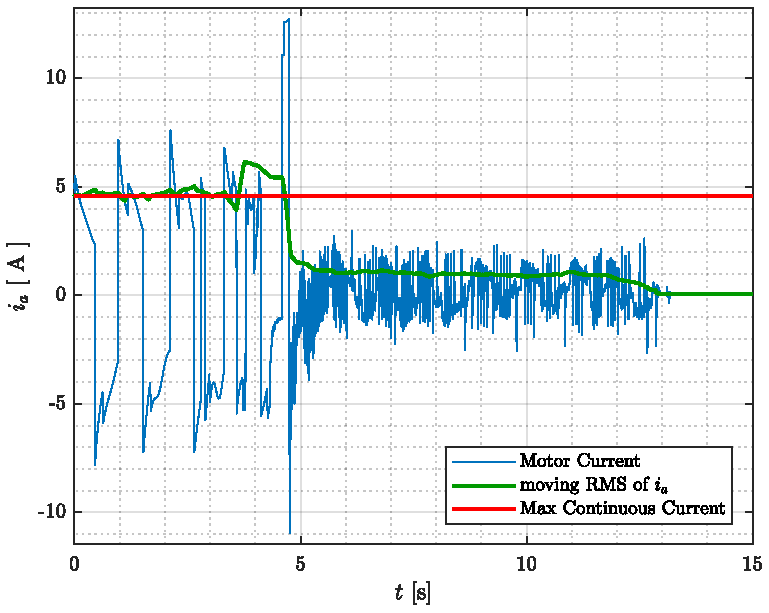
\includegraphics[width=.42\textwidth]{figures/ia_swingNslide}
  \caption{Armature current of the finished control system. It only briefly exceeds the motor specifications when the sliding mode controller takes over.}
  \label{fig:ia_swingNslide}
\end{figure}
%
Three energy based swing-up designs were investigated, the sat-based version was chosen, a cart position controller was added and finally a stabilizing sliding mode controller was designed to catch the pendulum in equilibrium. The design were successfully implemented and tested on the system setup whish concludes \textit{Part 1} of this thesis.